\section{BẢO MẬT TRONG HỆ CƠ SỞ DỮ LIỆU}
\label{sec:chuong6}

\subsection{Vì sao cần bảo mật}
\label{subsec:visao}

Bảo mật cơ sở dữ liệu là bảo vệ dữ liệu khỏi việc bị xem, sửa hoặc xóa bởi người không có quyền, đồng thời đảm bảo người có quyền vẫn dùng được dữ liệu khi cần. Các tài liệu về an toàn thông tin thường nêu ba mục tiêu là tính bí mật (confidentiality), tính toàn vẹn (integrity) và tính sẵn sàng (availability) \cite{elmasri}.

Với bài toán của nhóm, vấn đề này đặc biệt quan trọng vì lược đồ có các trường thông tin cá nhân như họ tên, ngày sinh, giới tính và nơi ở. Đây là loại dữ liệu thuộc phạm vi điều chỉnh của Luật Bảo vệ dữ liệu cá nhân số 91/2025/QH15, có hiệu lực từ ngày 01/01/2026 \cite{luat91}, và Nghị định 356/2025/NĐ-CP quy định chi tiết luật này, có hiệu lực cùng ngày; Nghị định 13/2023/NĐ-CP trước đây đã hết hiệu lực kể từ ngày Nghị định 356/2025/NĐ-CP có hiệu lực \cite{nd356}. Báo cáo chỉ nêu các văn bản này làm căn cứ cho việc phải bảo vệ dữ liệu, không phân tích nghĩa vụ pháp lý cụ thể của từng chủ thể. Bên cạnh đó, bảng bien\_dong\_cu\_tru đóng vai trò như một cuốn sổ ghi chép chính thức, nếu ai đó sửa hoặc xóa được thì lịch sử cư trú sẽ không còn đáng tin.

\subsection{Các cơ chế bảo mật thường dùng}
\label{subsec:coche}

\begin{table}[H]
\centering
\fontsize{12pt}{16pt}\selectfont
\renewcommand{\arraystretch}{1.15}
\begin{tabularx}{\textwidth}{|P{3.4cm}|Y|P{4.6cm}|}
\hline
\textbf{Cơ chế} & \textbf{Nội dung} & \textbf{Trong PostgreSQL} \\
\hline
Xác thực (authentication) & Kiểm tra người đăng nhập có đúng là người đó không & Role có thuộc tính LOGIN, mật khẩu băm SCRAM-SHA-256, cấu hình \texttt{pg\_hba.conf} \\
\hline
Phân quyền (authorization) & Quy định mỗi người được làm gì trên bảng nào & GRANT, REVOKE, ROLE, nguyên tắc quyền tối thiểu \\
\hline
Khung nhìn (view) & Chỉ cho xem một phần cột hoặc dòng của bảng & CREATE VIEW, tùy chọn \texttt{security\_invoker} \\
\hline
Bảo mật mức dòng & Mỗi người chỉ thấy các dòng được phép & Row-Level Security (CREATE POLICY) \\
\hline
Mã hóa (encryption) & Làm dữ liệu vô nghĩa nếu bị nghe lén hoặc lộ bản sao lưu & SSL/TLS khi kết nối, extension \texttt{pgcrypto} \\
\hline
Kiểm toán và sao lưu & Ghi lại ai đã làm gì; khôi phục khi mất dữ liệu & Cột thời điểm ghi, trigger, \texttt{pg\_dump} / \texttt{pg\_restore} \\
\hline
\end{tabularx}
\caption{Các cơ chế bảo mật cơ sở dữ liệu thường dùng}
\label{tab:coche}
\end{table}

Trong thiết kế của nhóm, bảng tai\_khoan không có cột mật khẩu (quy tắc B18). Việc xác thực do chính PostgreSQL đảm nhận qua các role có quyền đăng nhập, và mật khẩu của role được PostgreSQL lưu dưới dạng băm SCRAM-SHA-256, không bao giờ nằm trong bảng dữ liệu hay trong mã nguồn. Cột vai\_tro của tai\_khoan chỉ mô tả người ghi nhận biến động, còn quyền thật sự được cấp qua role của PostgreSQL.

\subsection{Ví dụ minh họa trên cơ sở dữ liệu cư trú}
\label{subsec:vidu}

Ví dụ 1 và 2 trình bày hai cách kiểm tra quyền trên cơ sở dữ liệu cư trú. Các đoạn mã minh họa đổi role bằng \texttt{SET ROLE}. Các ảnh bên dưới ghi lại phiên đăng nhập độc lập bằng từng role trên PostgreSQL 17.11, với \texttt{session\_user} và \texttt{current\_user} cùng mang tên role đã đăng nhập. Ví dụ 3 dành cho chức năng tra cứu. Mục \ref{subsec:danhgia} tổng hợp kết quả kiểm thử của cả chương \cite{postgres}.

\textbf{Ví dụ 1: Phân quyền theo nguyên tắc quyền tối thiểu và bảo vệ lịch sử (B1).} Nhóm tạo hai role đăng nhập độc lập, không phải superuser và không sở hữu bảng nào. Role \texttt{csdl17\_admin} được đọc và ghi dữ liệu nghiệp vụ nhưng bị thu hồi quyền DELETE trên hai bảng lịch sử (B12). Role \texttt{csdl17\_reader} là cán bộ tra cứu, chỉ được đọc sáu bảng nghiệp vụ và không được đọc bảng tài khoản.

\begin{lstlisting}[style=sqlvn]
CREATE ROLE csdl17_admin  LOGIN NOSUPERUSER NOCREATEDB NOCREATEROLE;
CREATE ROLE csdl17_reader LOGIN NOSUPERUSER NOCREATEDB NOCREATEROLE;

REVOKE ALL ON ALL TABLES IN SCHEMA public FROM PUBLIC;
GRANT USAGE ON SCHEMA public TO csdl17_admin, csdl17_reader;

-- Quản trị demo: đọc/ghi dữ liệu nghiệp vụ, nhưng không được xóa lịch sử (B12)
GRANT SELECT, INSERT, UPDATE, DELETE ON ALL TABLES IN SCHEMA public TO csdl17_admin;
GRANT USAGE, SELECT ON ALL SEQUENCES IN SCHEMA public TO csdl17_admin;
REVOKE DELETE ON qua_trinh_cu_tru, bien_dong_cu_tru FROM csdl17_admin;

-- Cán bộ tra cứu: chỉ đọc 6 bảng nghiệp vụ, không đọc bảng tài khoản
GRANT SELECT ON to_dan_pho, dia_chi, ho_cu_tru, cu_dan,
                qua_trinh_cu_tru, bien_dong_cu_tru TO csdl17_reader;

-- Thử quyền
SET ROLE csdl17_reader;
SELECT COUNT(*) FROM cu_dan;                                -- được phép: 200
UPDATE cu_dan SET ho_ten = 'Thử sửa' WHERE ma_cu_dan = 1;   -- bị từ chối
RESET ROLE;

SET ROLE csdl17_admin;
DELETE FROM bien_dong_cu_tru WHERE ma_bien_dong = 1;        -- bị từ chối
RESET ROLE;
\end{lstlisting}

Hình~\ref{fig:sec-b1-select} cho thấy role \texttt{csdl17\_reader} đếm được 200 cư dân. Hình~\ref{fig:sec-b1-denied} ghi nhận PostgreSQL từ chối thao tác ghi và đọc bảng tài khoản trong phiên của cùng role. Nhật ký kiểm thử ghi mã SQLSTATE 42501 cho các trường hợp này.

Trong phép thử B1, PostgreSQL từ chối lệnh \texttt{DELETE} trên bảng biến động khi chạy dưới role \texttt{csdl17\_admin}. Kết quả xác nhận cơ chế thu hồi quyền xóa bản ghi theo B12.

\begin{figure}[H]
    \centering
    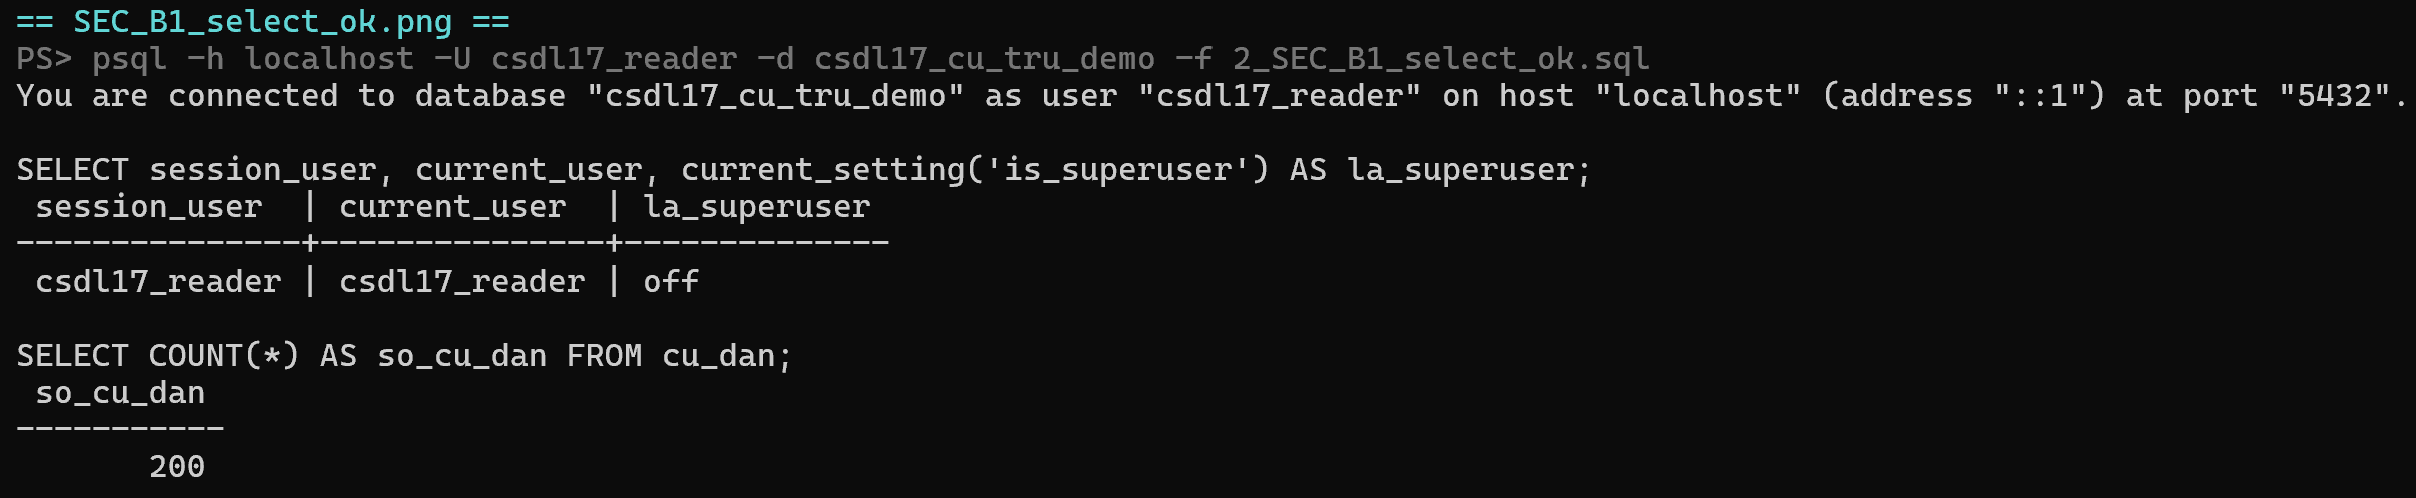
\includegraphics[trim=0bp 0bp 223bp 50bp,clip,width=\linewidth]{image/security/SEC_B1_select_ok.png}
    \caption{B1 --- Role tra cứu đăng nhập độc lập và đếm được 200 cư dân}
    \label{fig:sec-b1-select}
    \par\medskip
    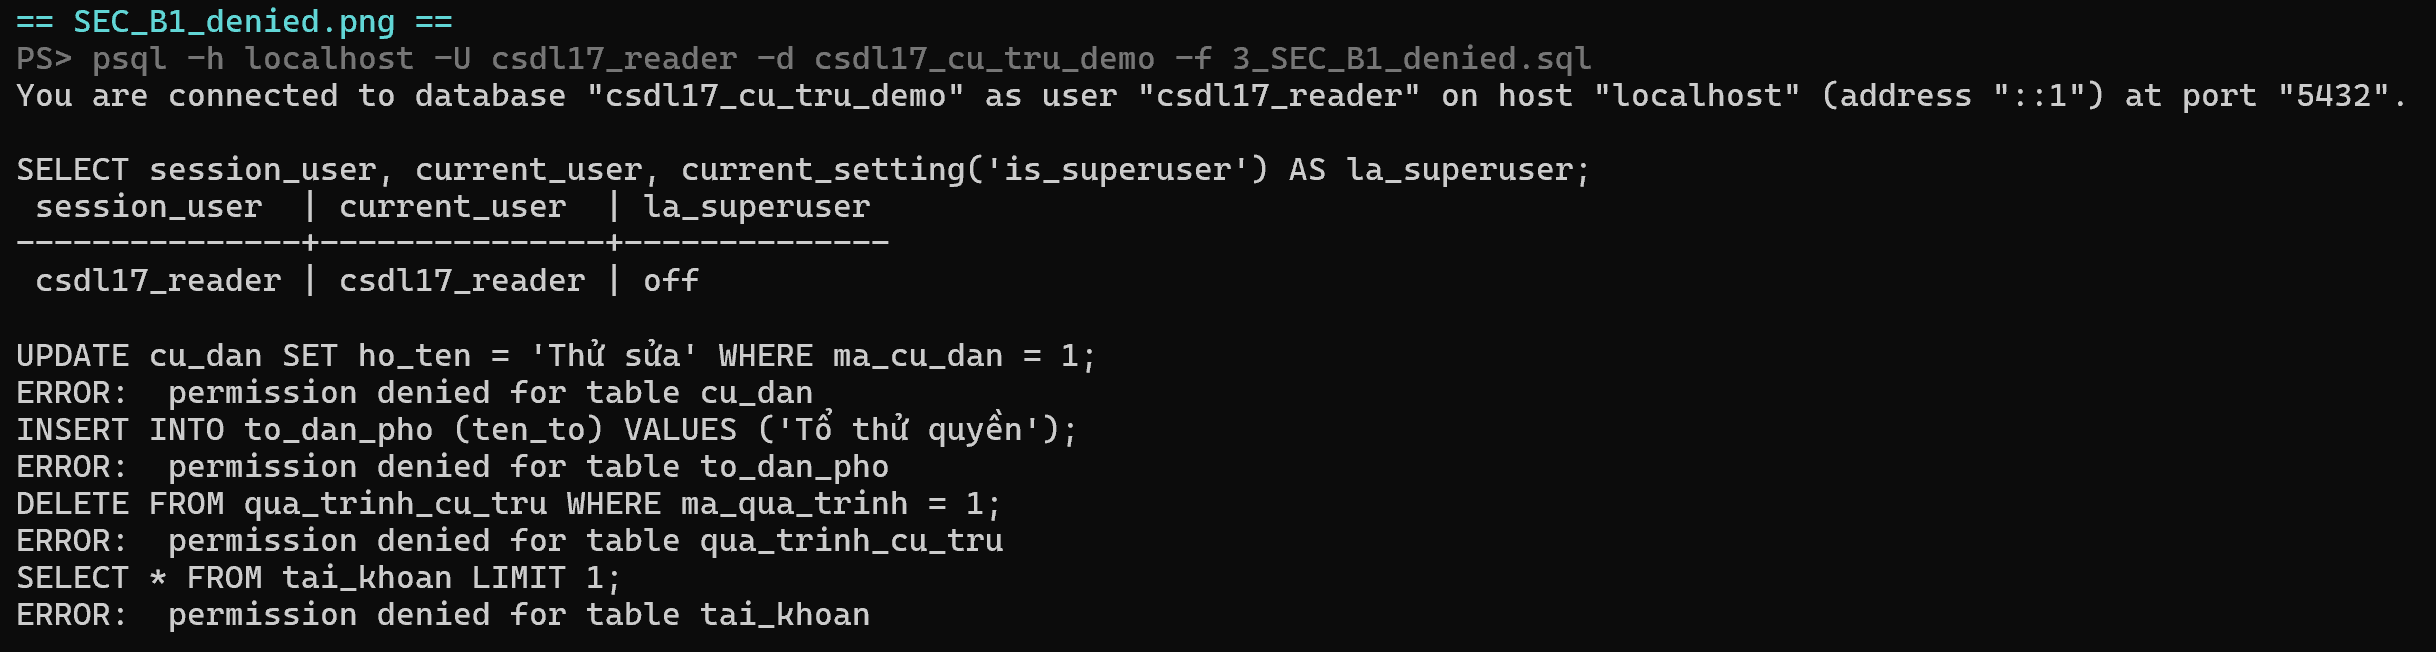
\includegraphics[trim=0bp 0bp 231bp 50bp,clip,width=\linewidth]{image/security/SEC_B1_denied.png}
    \caption{B1 --- PostgreSQL từ chối thao tác ghi và đọc bảng tài khoản}
    \label{fig:sec-b1-denied}
\end{figure}

\textbf{Ví dụ 2: Dùng khung nhìn để chỉ công bố số liệu tổng hợp (B2).} Cán bộ tổng hợp của phường cần biết mỗi tổ đang có bao nhiêu người cư trú, nhưng không cần biết họ tên hay ngày sinh của từng người. Nhóm tạo một view chỉ trả về mã tổ, tên tổ và số người, rồi chỉ cấp quyền trên view này cho role \texttt{csdl17\_report}, không cấp quyền trên bảng gốc.

\begin{lstlisting}[style=sqlvn]
CREATE ROLE csdl17_report LOGIN NOSUPERUSER NOCREATEDB NOCREATEROLE;
GRANT USAGE ON SCHEMA public TO csdl17_report;

CREATE VIEW vw_thong_ke_cu_dan_theo_to
WITH (security_invoker = false) AS
SELECT t.ma_to,
       t.ten_to,
       COUNT(DISTINCT q.ma_cu_dan) AS so_cu_dan
FROM to_dan_pho t
LEFT JOIN dia_chi d          ON d.ma_to = t.ma_to
LEFT JOIN ho_cu_tru h        ON h.ma_dia_chi = d.ma_dia_chi
LEFT JOIN qua_trinh_cu_tru q ON q.ma_ho = h.ma_ho
                            AND q.ngay_bat_dau <= CURRENT_DATE
                            AND (q.ngay_ket_thuc IS NULL
                                 OR q.ngay_ket_thuc >= CURRENT_DATE)
GROUP BY t.ma_to, t.ten_to;

GRANT SELECT ON vw_thong_ke_cu_dan_theo_to TO csdl17_report;

SET ROLE csdl17_report;
SELECT * FROM vw_thong_ke_cu_dan_theo_to ORDER BY ma_to;    -- được phép
SELECT ho_ten, ngay_sinh FROM cu_dan LIMIT 1;               -- bị từ chối
RESET ROLE;
\end{lstlisting}

Hình~\ref{fig:sec-b2-view} cho thấy \texttt{csdl17\_report} đọc được VIEW gồm ba cột và tám tổ. Trong lần chạy này, Tổ 01 có 34 cư dân và Tổ 08 có 0. PostgreSQL từ chối quyền đọc trực tiếp hai bảng gốc \texttt{cu\_dan} và \texttt{qua\_trinh\_cu\_tru} trong cùng role (Hình~\ref{fig:sec-b2-denied}). Điều này làm được nhờ tùy chọn \texttt{security\_invoker = false}: view đọc các bảng nền bằng quyền của chủ sở hữu view, nên người dùng chỉ cần quyền trên view mà không cần quyền trên từng bảng bên dưới. Khung nhìn công bố ba trường tổng hợp và ẩn các trường định danh cư dân.

\begin{figure}[H]
    \centering
    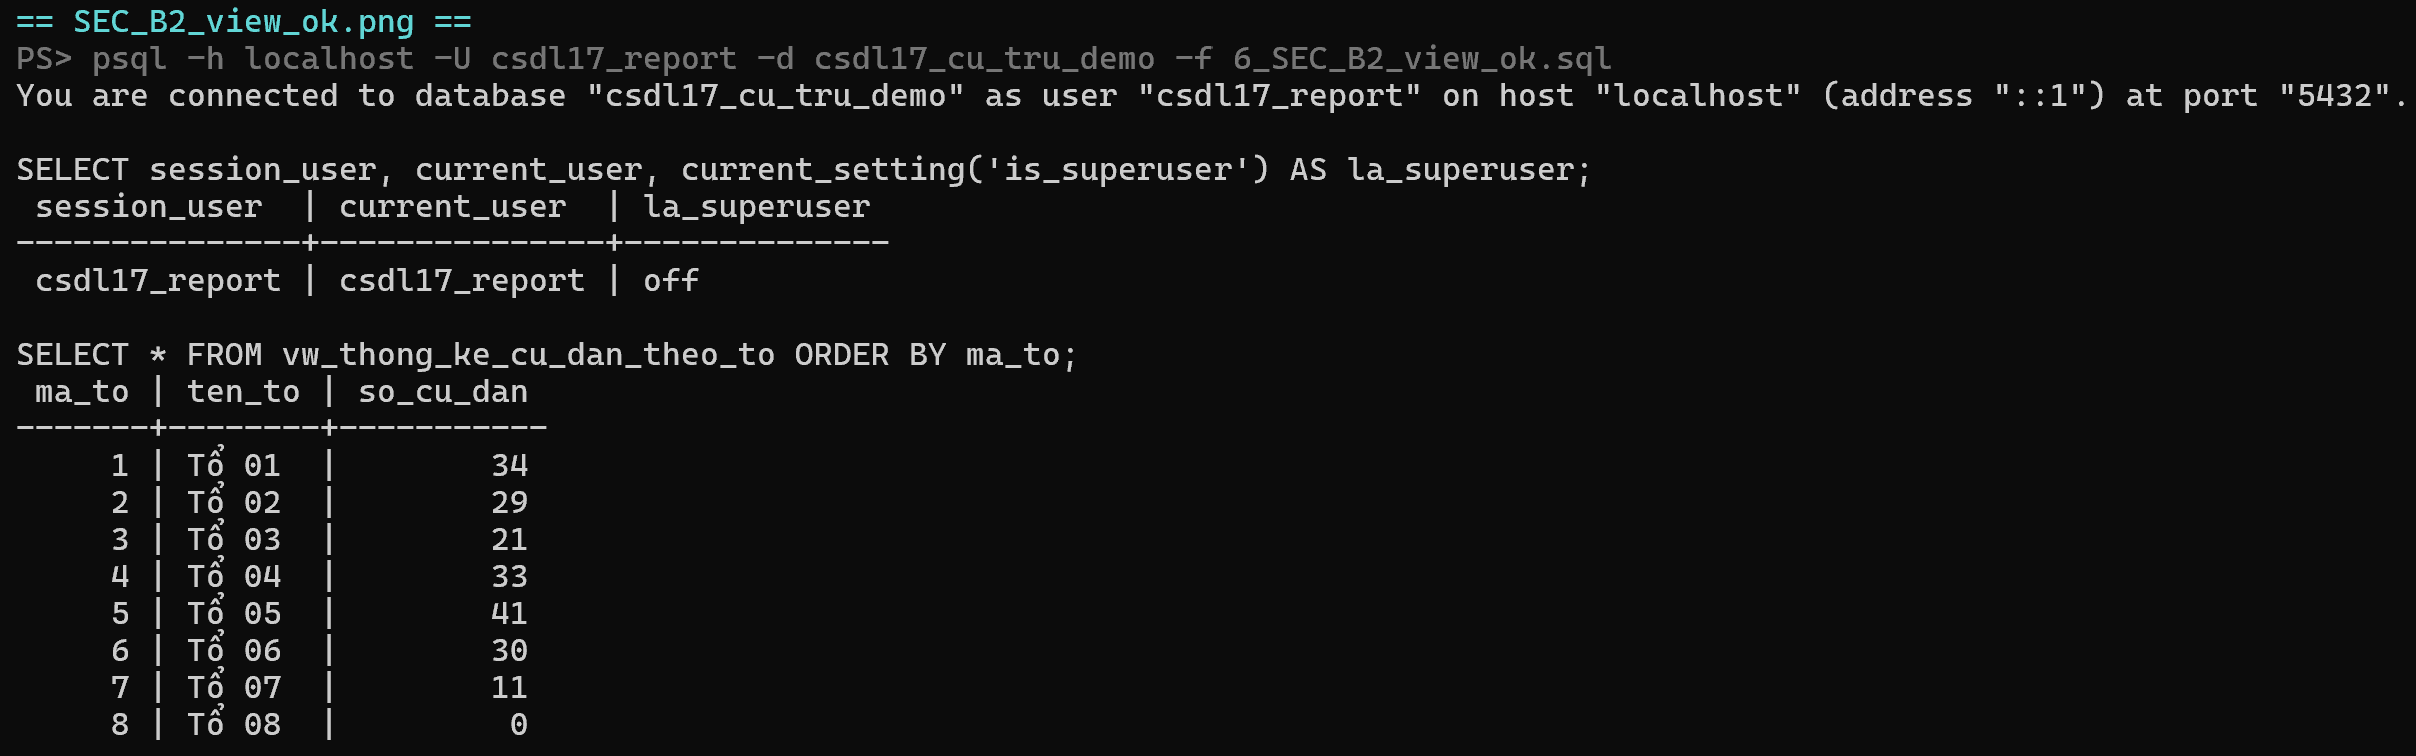
\includegraphics[trim=0bp 0bp 223bp 50bp,clip,width=\linewidth]{image/security/SEC_B2_view_ok.png}
    \caption{B2 --- Role báo cáo đăng nhập độc lập và đọc được VIEW}
    \label{fig:sec-b2-view}
    \par\medskip
    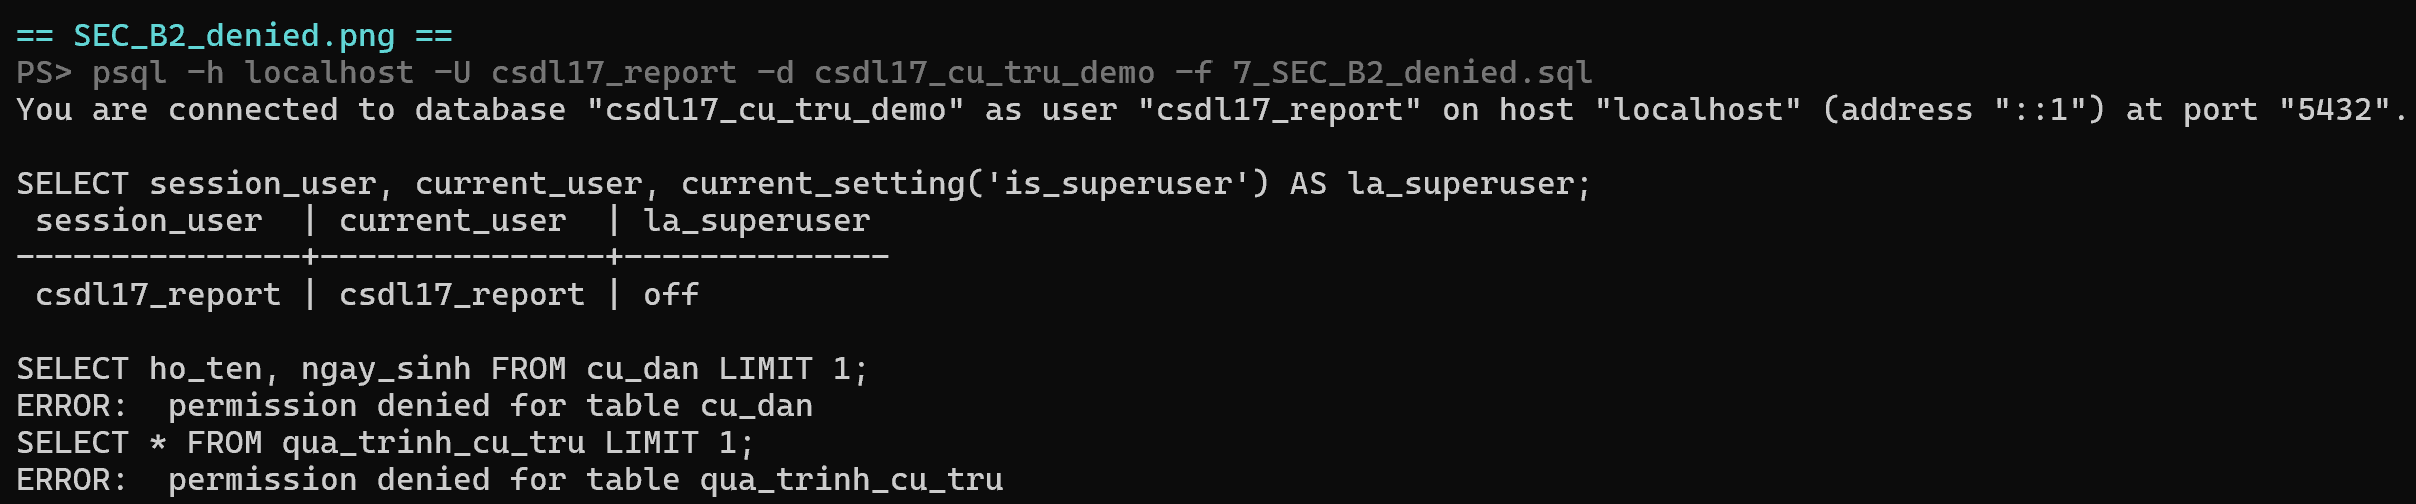
\includegraphics[trim=0bp 0bp 223bp 50bp,clip,width=\linewidth]{image/security/SEC_B2_denied.png}
    \caption{B2 --- PostgreSQL từ chối quyền đọc trực tiếp hai bảng gốc}
    \label{fig:sec-b2-denied}
\end{figure}

\textbf{Ví dụ 3: Chống tấn công SQL Injection ở chức năng tra cứu cư dân.} Chức năng tra cứu cho phép cán bộ gõ một phần họ tên để tìm cư dân. Nếu lập trình viên ghép thẳng chuỗi người dùng nhập vào một câu lệnh động như dưới đây thì kẻ xấu có thể chèn thêm mã SQL của họ.

\begin{lstlisting}[style=sqlvn]
-- CÁCH VIẾT SAI: ghép chuỗi người dùng nhập vào câu lệnh động
CREATE FUNCTION fn_tim_cu_dan_sai(p_ten TEXT)
RETURNS TABLE (ma_cu_dan BIGINT, ho_ten VARCHAR, ngay_sinh DATE)
LANGUAGE plpgsql AS $$
BEGIN
    RETURN QUERY EXECUTE
        'SELECT ma_cu_dan, ho_ten, ngay_sinh FROM cu_dan WHERE ho_ten LIKE ''%'
        || p_ten || '%''';
END;
$$;

SELECT COUNT(*) FROM fn_tim_cu_dan_sai('x'' OR 1=1 --');
-- Câu lệnh thực sự chạy là:
--   ... WHERE ho_ten LIKE '%x' OR 1=1 --%'
-- điều kiện 1=1 luôn đúng nên trả về toàn bộ 200 cư dân
\end{lstlisting}

Cách khắc phục là để giá trị người dùng nhập vào chỉ đóng vai trò tham số. Khi viết hàm bằng SQL thuần, PostgreSQL luôn coi \texttt{p\_ten} là dữ liệu cần so khớp, không bao giờ coi nó là một phần của câu lệnh. Nếu bắt buộc phải dùng câu lệnh động, cần truyền giá trị qua \texttt{EXECUTE \ldots{} USING} hoặc định dạng bằng \texttt{format('\%L', \ldots)} chứ không ghép chuỗi.

\begin{lstlisting}[style=sqlvn]
-- CÁCH VIẾT ĐÚNG: giá trị nhập vào chỉ được dùng như một tham số
CREATE FUNCTION fn_tim_cu_dan(p_ten TEXT)
RETURNS TABLE (ma_cu_dan BIGINT, ho_ten VARCHAR, ngay_sinh DATE)
LANGUAGE sql STABLE AS $$
    SELECT c.ma_cu_dan, c.ho_ten, c.ngay_sinh
    FROM cu_dan c
    WHERE c.ho_ten LIKE '%' || p_ten || '%';
$$;

REVOKE EXECUTE ON FUNCTION fn_tim_cu_dan(TEXT) FROM PUBLIC;
GRANT  EXECUTE ON FUNCTION fn_tim_cu_dan(TEXT) TO csdl17_reader;

SELECT COUNT(*) FROM fn_tim_cu_dan('x'' OR 1=1 --');   -- 0 dòng
SELECT COUNT(*) FROM fn_tim_cu_dan('Hùng');            -- 8 dòng
\end{lstlisting}

Với cùng chuỗi tấn công, hàm viết đúng chỉ tìm người có họ tên chứa đúng chuỗi ký tự đó và trả về 0 dòng, trong khi tìm theo tên ``Hùng'' vẫn ra đúng 8 cư dân. Ngoài ra, việc thu hồi quyền EXECUTE mặc định của PUBLIC rồi chỉ cấp cho csdl17\_reader cũng giúp giới hạn ai được gọi hàm tra cứu: khi chạy thử, csdl17\_reader gọi được hàm, còn csdl17\_report bị từ chối với thông báo \textit{permission denied for function fn\_tim\_cu\_dan}.

Hai hàm của Ví dụ 3 không nằm trong các script cài đặt của nhóm. Nhóm chỉ tạo chúng trên một cơ sở dữ liệu thử nghiệm riêng, trong một giao dịch kết thúc bằng ROLLBACK, để đo các con số 200, 0 và 8 ở trên; hàm viết sai chỉ dùng để minh họa lỗ hổng và không được đưa vào môi trường vận hành.

\subsection{Đánh giá kết quả và giới hạn bảo mật}
\label{subsec:danhgia}

\textbf{Kết quả kiểm thử.} Nhóm kiểm tra cấu hình quyền, thao tác được phép và thao tác bị từ chối; mỗi phép thử đối chiếu kết quả kỳ vọng với kết quả thực tế. Bảng \ref{tab:ketquabaomat} tóm tắt kết quả. Các kiểm thử đã được thực hiện trên PostgreSQL 17.11 với Windows 11 và PostgreSQL 17.12 với CSDL thử nghiệm dựng mới. Phiên đăng nhập độc lập qua TCP được kiểm tra với SCRAM-SHA-256; phép thử cục bộ không dùng mật khẩu chỉ áp dụng trong cụm tạm biệt lập. Script và log chi tiết được lưu trong hồ sơ kiểm thử của dự án.

\begin{table}[H]
\centering
\fontsize{11pt}{14pt}\selectfont
\renewcommand{\arraystretch}{1.15}
\begin{tabularx}{\textwidth}{|P{3.6cm}|Y|P{2.1cm}|}
\hline
\textbf{Kiểm thử (tệp)} & \textbf{Nội dung kiểm tra} & \textbf{Kết quả} \\
\hline
Kiểm tra quyền đã cấp (\texttt{security\_catalog\_tv3.sql}) & Ba role demo không đặc quyền, không sở hữu đối tượng, không là thành viên role khác; PUBLIC không có CONNECT/TEMP/CREATE và không có quyền trên bảng; reader chỉ đọc 6 bảng; report chỉ đọc VIEW; VIEW không có cột định danh; admin không có DELETE trên hai bảng lịch sử & 15/15 PASS \\
\hline
Đăng nhập thật bằng csdl17\_reader (\texttt{security\_login\_tv3.sql}) & SELECT được; UPDATE, INSERT, DELETE, TRUNCATE, đọc tai\_khoan, đọc VIEW, gọi \texttt{fn\_chuyen\_noi\_bo}, tạo bảng, tạo bảng tạm và SET ROLE sang admin đều bị từ chối (42501) & 12/12 PASS \\
\hline
Đăng nhập thật bằng csdl17\_report (\texttt{security\_login\_tv3.sql}) & Đọc VIEW được (8 tổ); đọc 4 bảng gốc, gọi hàm, tạo bảng, SET ROLE bị từ chối (42501); ghi VIEW báo 55000 vì VIEW có GROUP BY & 10/10 PASS \\
\hline
Bảo vệ lịch sử B12 (\texttt{security\_b12\_tv1.sql}) & Ma trận 3 role $\times$ 8 đối tượng $\times$ 5 quyền khớp thiết kế; admin DELETE, TRUNCATE hai bảng lịch sử bị từ chối; admin vẫn chạy được \texttt{fn\_chuyen\_noi\_bo} & K01--K05 PASS \\
\hline
Ví dụ của chương và quyền admin (\texttt{report\_security\_ch6.sql}) & Kết quả của Ví dụ 1--3 và các phép thử giới hạn quyền csdl17\_admin nêu dưới đây & Đúng như mô tả \\
\hline
\end{tabularx}
\caption{Tóm tắt kết quả kiểm thử bảo mật}
\label{tab:ketquabaomat}
\end{table}

Khác với \texttt{SET ROLE} ở Ví dụ 1 và 2, các phép thử đăng nhập thật mở phiên mới bằng \texttt{psql -h localhost -U csdl17\_reader} (tương tự với csdl17\_report). Dòng đầu mỗi log xác nhận \texttt{session\_user} và \texttt{current\_user} đều là role demo và phiên không phải superuser, nên kết quả phản ánh đúng quyền của role khi được dùng độc lập. Mật khẩu tạm chỉ đặt cho phiên thử và được xóa ngay sau đó, không ghi vào mã nguồn. Sau các phiên thử, giá trị băm md5 của các bảng dữ liệu không đổi. Các ảnh bổ trợ về quyền, dữ liệu trước và sau phép thử, và định nghĩa VIEW nằm trong \hyperref[sec:anh-sec]{phụ lục ảnh kiểm thử bảo mật}.

\textbf{Giới hạn của quyền csdl17\_admin.} Các phép thử trong giao dịch có \texttt{ROLLBACK} cho kết quả sau.
\begin{itemize}[leftmargin=*]
    \item \textbf{Vẫn sửa được lịch sử trong phạm vi trigger cho phép.} csdl17\_admin sửa được ghi chú của một biến động, đổi tài khoản ghi nhận của biến động cũ sang một tài khoản đang hoạt động khác, và đóng một đợt cư trú chưa gắn với biến động nào. Các lệnh làm sai quan hệ ngày giữa biến động và đợt cư trú, như đổi ngày biến động hay sửa ngày kết thúc của đợt đã gắn biến động, bị trigger B09 chặn với SQLSTATE 23514.
    \item \textbf{Quyền trên bảng tài khoản.} Role \texttt{csdl17\_admin} có quyền đọc, thêm, sửa và xóa bản ghi trên bảng \texttt{tai\_khoan}. Xóa tài khoản đã ghi biến động bị khóa ngoại chặn (23503), nhưng tài khoản chưa ghi biến động nào (tài khoản 5) thì xóa được. Admin cũng sửa được ten\_hien\_thi, vai\_tro và trang\_thai. Do nhật ký biến động chỉ lưu ma\_tai\_khoan, đổi tên hiển thị sẽ đổi cách đọc ``ai đã ghi'' của các biến động cũ; còn mở khóa một tài khoản đang KHOA thì tài khoản đó ghi lại được ngay, vì B14 chỉ kiểm tra trạng thái tại thời điểm ghi.
    \item \textbf{Vai trò nghiệp vụ chỉ là nhãn mô tả (X01, phương án b).} Cột tai\_khoan.vai\_tro chỉ là nhãn mô tả người ghi; quyền thực tế do role PostgreSQL quyết định, và trigger B14 chỉ kiểm tra tài khoản đang HOAT\_DONG chứ không kiểm tra vai trò. Bộ dữ liệu mẫu được giữ nguyên: 13/63 biến động do tài khoản có vai trò THONG\_KE ghi và 11/63 do tài khoản QUAN\_TRI ghi.
\end{itemize}

\textbf{Các giới hạn khác.} VIEW tổng hợp vẫn có nguy cơ suy luận ở nhóm nhỏ. Thống kê hiện tại dùng ngày hệ thống nên kết quả thay đổi theo thời gian. Đồ án chưa triển khai bảo mật mức dòng, kiểm toán đầy đủ, mã hóa kết nối TLS hay chính sách \texttt{pg\_hba.conf} cho vận hành. Các hàm \texttt{fn\_*} vẫn cho PUBLIC quyền EXECUTE nhưng chạy với quyền người gọi (SECURITY INVOKER); nếu đổi sang SECURITY DEFINER, phải rà soát và thu hồi quyền PUBLIC phù hợp.
